% Options for packages loaded elsewhere
\PassOptionsToPackage{unicode}{hyperref}
\PassOptionsToPackage{hyphens}{url}
\PassOptionsToPackage{dvipsnames,svgnames,x11names}{xcolor}
%
\documentclass[
  letterpaper,
  DIV=11,
  numbers=noendperiod]{scrartcl}

\usepackage{amsmath,amssymb}
\usepackage{iftex}
\ifPDFTeX
  \usepackage[T1]{fontenc}
  \usepackage[utf8]{inputenc}
  \usepackage{textcomp} % provide euro and other symbols
\else % if luatex or xetex
  \usepackage{unicode-math}
  \defaultfontfeatures{Scale=MatchLowercase}
  \defaultfontfeatures[\rmfamily]{Ligatures=TeX,Scale=1}
\fi
\usepackage{lmodern}
\ifPDFTeX\else  
    % xetex/luatex font selection
\fi
% Use upquote if available, for straight quotes in verbatim environments
\IfFileExists{upquote.sty}{\usepackage{upquote}}{}
\IfFileExists{microtype.sty}{% use microtype if available
  \usepackage[]{microtype}
  \UseMicrotypeSet[protrusion]{basicmath} % disable protrusion for tt fonts
}{}
\makeatletter
\@ifundefined{KOMAClassName}{% if non-KOMA class
  \IfFileExists{parskip.sty}{%
    \usepackage{parskip}
  }{% else
    \setlength{\parindent}{0pt}
    \setlength{\parskip}{6pt plus 2pt minus 1pt}}
}{% if KOMA class
  \KOMAoptions{parskip=half}}
\makeatother
\usepackage{xcolor}
\setlength{\emergencystretch}{3em} % prevent overfull lines
\setcounter{secnumdepth}{-\maxdimen} % remove section numbering
% Make \paragraph and \subparagraph free-standing
\ifx\paragraph\undefined\else
  \let\oldparagraph\paragraph
  \renewcommand{\paragraph}[1]{\oldparagraph{#1}\mbox{}}
\fi
\ifx\subparagraph\undefined\else
  \let\oldsubparagraph\subparagraph
  \renewcommand{\subparagraph}[1]{\oldsubparagraph{#1}\mbox{}}
\fi

\usepackage{color}
\usepackage{fancyvrb}
\newcommand{\VerbBar}{|}
\newcommand{\VERB}{\Verb[commandchars=\\\{\}]}
\DefineVerbatimEnvironment{Highlighting}{Verbatim}{commandchars=\\\{\}}
% Add ',fontsize=\small' for more characters per line
\usepackage{framed}
\definecolor{shadecolor}{RGB}{241,243,245}
\newenvironment{Shaded}{\begin{snugshade}}{\end{snugshade}}
\newcommand{\AlertTok}[1]{\textcolor[rgb]{0.68,0.00,0.00}{#1}}
\newcommand{\AnnotationTok}[1]{\textcolor[rgb]{0.37,0.37,0.37}{#1}}
\newcommand{\AttributeTok}[1]{\textcolor[rgb]{0.40,0.45,0.13}{#1}}
\newcommand{\BaseNTok}[1]{\textcolor[rgb]{0.68,0.00,0.00}{#1}}
\newcommand{\BuiltInTok}[1]{\textcolor[rgb]{0.00,0.23,0.31}{#1}}
\newcommand{\CharTok}[1]{\textcolor[rgb]{0.13,0.47,0.30}{#1}}
\newcommand{\CommentTok}[1]{\textcolor[rgb]{0.37,0.37,0.37}{#1}}
\newcommand{\CommentVarTok}[1]{\textcolor[rgb]{0.37,0.37,0.37}{\textit{#1}}}
\newcommand{\ConstantTok}[1]{\textcolor[rgb]{0.56,0.35,0.01}{#1}}
\newcommand{\ControlFlowTok}[1]{\textcolor[rgb]{0.00,0.23,0.31}{#1}}
\newcommand{\DataTypeTok}[1]{\textcolor[rgb]{0.68,0.00,0.00}{#1}}
\newcommand{\DecValTok}[1]{\textcolor[rgb]{0.68,0.00,0.00}{#1}}
\newcommand{\DocumentationTok}[1]{\textcolor[rgb]{0.37,0.37,0.37}{\textit{#1}}}
\newcommand{\ErrorTok}[1]{\textcolor[rgb]{0.68,0.00,0.00}{#1}}
\newcommand{\ExtensionTok}[1]{\textcolor[rgb]{0.00,0.23,0.31}{#1}}
\newcommand{\FloatTok}[1]{\textcolor[rgb]{0.68,0.00,0.00}{#1}}
\newcommand{\FunctionTok}[1]{\textcolor[rgb]{0.28,0.35,0.67}{#1}}
\newcommand{\ImportTok}[1]{\textcolor[rgb]{0.00,0.46,0.62}{#1}}
\newcommand{\InformationTok}[1]{\textcolor[rgb]{0.37,0.37,0.37}{#1}}
\newcommand{\KeywordTok}[1]{\textcolor[rgb]{0.00,0.23,0.31}{#1}}
\newcommand{\NormalTok}[1]{\textcolor[rgb]{0.00,0.23,0.31}{#1}}
\newcommand{\OperatorTok}[1]{\textcolor[rgb]{0.37,0.37,0.37}{#1}}
\newcommand{\OtherTok}[1]{\textcolor[rgb]{0.00,0.23,0.31}{#1}}
\newcommand{\PreprocessorTok}[1]{\textcolor[rgb]{0.68,0.00,0.00}{#1}}
\newcommand{\RegionMarkerTok}[1]{\textcolor[rgb]{0.00,0.23,0.31}{#1}}
\newcommand{\SpecialCharTok}[1]{\textcolor[rgb]{0.37,0.37,0.37}{#1}}
\newcommand{\SpecialStringTok}[1]{\textcolor[rgb]{0.13,0.47,0.30}{#1}}
\newcommand{\StringTok}[1]{\textcolor[rgb]{0.13,0.47,0.30}{#1}}
\newcommand{\VariableTok}[1]{\textcolor[rgb]{0.07,0.07,0.07}{#1}}
\newcommand{\VerbatimStringTok}[1]{\textcolor[rgb]{0.13,0.47,0.30}{#1}}
\newcommand{\WarningTok}[1]{\textcolor[rgb]{0.37,0.37,0.37}{\textit{#1}}}

\providecommand{\tightlist}{%
  \setlength{\itemsep}{0pt}\setlength{\parskip}{0pt}}\usepackage{longtable,booktabs,array}
\usepackage{calc} % for calculating minipage widths
% Correct order of tables after \paragraph or \subparagraph
\usepackage{etoolbox}
\makeatletter
\patchcmd\longtable{\par}{\if@noskipsec\mbox{}\fi\par}{}{}
\makeatother
% Allow footnotes in longtable head/foot
\IfFileExists{footnotehyper.sty}{\usepackage{footnotehyper}}{\usepackage{footnote}}
\makesavenoteenv{longtable}
\usepackage{graphicx}
\makeatletter
\def\maxwidth{\ifdim\Gin@nat@width>\linewidth\linewidth\else\Gin@nat@width\fi}
\def\maxheight{\ifdim\Gin@nat@height>\textheight\textheight\else\Gin@nat@height\fi}
\makeatother
% Scale images if necessary, so that they will not overflow the page
% margins by default, and it is still possible to overwrite the defaults
% using explicit options in \includegraphics[width, height, ...]{}
\setkeys{Gin}{width=\maxwidth,height=\maxheight,keepaspectratio}
% Set default figure placement to htbp
\makeatletter
\def\fps@figure{htbp}
\makeatother

\KOMAoption{captions}{tableheading}
\makeatletter
\@ifpackageloaded{caption}{}{\usepackage{caption}}
\AtBeginDocument{%
\ifdefined\contentsname
  \renewcommand*\contentsname{Table of contents}
\else
  \newcommand\contentsname{Table of contents}
\fi
\ifdefined\listfigurename
  \renewcommand*\listfigurename{List of Figures}
\else
  \newcommand\listfigurename{List of Figures}
\fi
\ifdefined\listtablename
  \renewcommand*\listtablename{List of Tables}
\else
  \newcommand\listtablename{List of Tables}
\fi
\ifdefined\figurename
  \renewcommand*\figurename{Figure}
\else
  \newcommand\figurename{Figure}
\fi
\ifdefined\tablename
  \renewcommand*\tablename{Table}
\else
  \newcommand\tablename{Table}
\fi
}
\@ifpackageloaded{float}{}{\usepackage{float}}
\floatstyle{ruled}
\@ifundefined{c@chapter}{\newfloat{codelisting}{h}{lop}}{\newfloat{codelisting}{h}{lop}[chapter]}
\floatname{codelisting}{Listing}
\newcommand*\listoflistings{\listof{codelisting}{List of Listings}}
\makeatother
\makeatletter
\makeatother
\makeatletter
\@ifpackageloaded{caption}{}{\usepackage{caption}}
\@ifpackageloaded{subcaption}{}{\usepackage{subcaption}}
\makeatother
\ifLuaTeX
  \usepackage{selnolig}  % disable illegal ligatures
\fi
\usepackage{bookmark}

\IfFileExists{xurl.sty}{\usepackage{xurl}}{} % add URL line breaks if available
\urlstyle{same} % disable monospaced font for URLs
\hypersetup{
  pdftitle={DLMs and GAMs for Lake Washington data},
  colorlinks=true,
  linkcolor={blue},
  filecolor={Maroon},
  citecolor={Blue},
  urlcolor={Blue},
  pdfcreator={LaTeX via pandoc}}

\title{DLMs and GAMs for Lake Washington data}
\author{}
\date{}

\begin{document}
\maketitle

\begin{Shaded}
\begin{Highlighting}[]
\CommentTok{\#install.packages(\textquotesingle{}marssTMB\textquotesingle{}, repos = c(\textquotesingle{}https://atsa{-}es.r{-}universe.dev\textquotesingle{}, \#\textquotesingle{}https://cloud.r{-}project.org\textquotesingle{}))}
\FunctionTok{library}\NormalTok{(MARSS)}
\FunctionTok{library}\NormalTok{(mgcv)}
\FunctionTok{library}\NormalTok{(dplyr)}
\FunctionTok{library}\NormalTok{(forecast)}
\FunctionTok{library}\NormalTok{(ggplot2)}
\FunctionTok{library}\NormalTok{(lubridate)}
\FunctionTok{library}\NormalTok{(marssTMB)}
\FunctionTok{library}\NormalTok{(paletteer)}
\NormalTok{col}\OtherTok{\textless{}{-}}\FunctionTok{paletteer\_d}\NormalTok{(}\StringTok{"nationalparkcolors::Everglades"}\NormalTok{)}
\end{Highlighting}
\end{Shaded}

\subsection{Data}\label{data}

\begin{Shaded}
\begin{Highlighting}[]
\NormalTok{dat\_lakewa }\OtherTok{\textless{}{-}} \FunctionTok{readRDS}\NormalTok{(}\StringTok{"data\_for\_lakeWA\_example.rds"}\NormalTok{)}
\NormalTok{dat\_aksalmon }\OtherTok{\textless{}{-}} \FunctionTok{readRDS}\NormalTok{(}\StringTok{"data\_for\_AK\_salmon\_example.rds"}\NormalTok{)}

\CommentTok{\# renaming}
\NormalTok{dat\_lakewa }\OtherTok{\textless{}{-}}\NormalTok{ dplyr}\SpecialCharTok{::}\FunctionTok{rename}\NormalTok{(dat\_lakewa, }
                            \AttributeTok{response =}\NormalTok{ y\_adj,}
                            \AttributeTok{driver =}\NormalTok{ lagged\_zp)}
\NormalTok{dat\_aksalmon }\OtherTok{\textless{}{-}}\NormalTok{ dplyr}\SpecialCharTok{::}\FunctionTok{rename}\NormalTok{(dat\_aksalmon,}
                              \AttributeTok{response =}\NormalTok{ salmon\_DFA,}
                              \AttributeTok{driver =}\NormalTok{ z\_sst, }
                              \AttributeTok{date =}\NormalTok{ year)}
\end{Highlighting}
\end{Shaded}

\subsection{DLM with time-varying intercepts and time-varying
slopes}\label{dlm-with-time-varying-intercepts-and-time-varying-slopes}

Define the model -- this block is basically copied from the MARSS book
(salmon survival case study). First for the Lake WA example:

\begin{Shaded}
\begin{Highlighting}[]
\NormalTok{dat }\OtherTok{\textless{}{-}}\NormalTok{ dat\_lakewa}
\NormalTok{m }\OtherTok{\textless{}{-}} \DecValTok{2}
\NormalTok{TT }\OtherTok{\textless{}{-}} \FunctionTok{nrow}\NormalTok{(dat)}
\NormalTok{B }\OtherTok{\textless{}{-}} \FunctionTok{diag}\NormalTok{(m)  }\DocumentationTok{\#\# 2x2; Identity}
\NormalTok{U }\OtherTok{\textless{}{-}} \FunctionTok{matrix}\NormalTok{(}\DecValTok{0}\NormalTok{, }\AttributeTok{nrow =}\NormalTok{ m, }\AttributeTok{ncol =} \DecValTok{1}\NormalTok{)  }\DocumentationTok{\#\# 2x1; both elements = 0}
\NormalTok{Q }\OtherTok{\textless{}{-}} \FunctionTok{matrix}\NormalTok{(}\FunctionTok{list}\NormalTok{(}\DecValTok{0}\NormalTok{), m, m)  }\DocumentationTok{\#\# 2x2; all 0 for now}
\FunctionTok{diag}\NormalTok{(Q)[}\DecValTok{1}\NormalTok{] }\OtherTok{\textless{}{-}} \FunctionTok{c}\NormalTok{(}\StringTok{"q.alpha"}\NormalTok{)}
\FunctionTok{diag}\NormalTok{(Q)[}\DecValTok{2}\NormalTok{] }\OtherTok{\textless{}{-}} \FunctionTok{c}\NormalTok{(}\StringTok{"q.beta"}\NormalTok{)}
\NormalTok{Z }\OtherTok{\textless{}{-}} \FunctionTok{array}\NormalTok{(}\ConstantTok{NA}\NormalTok{, }\FunctionTok{c}\NormalTok{(}\DecValTok{1}\NormalTok{, m, TT))  }\DocumentationTok{\#\# NxMxT; empty for now}
\NormalTok{Z[}\DecValTok{1}\NormalTok{, }\DecValTok{1}\NormalTok{, ] }\OtherTok{\textless{}{-}} \FunctionTok{rep}\NormalTok{(}\DecValTok{1}\NormalTok{, TT)  }\DocumentationTok{\#\# Nx1; 1\textquotesingle{}s for intercept}
\NormalTok{Z[}\DecValTok{1}\NormalTok{, }\DecValTok{2}\NormalTok{, ] }\OtherTok{\textless{}{-}}\NormalTok{ dat}\SpecialCharTok{$}\NormalTok{driver  }\DocumentationTok{\#\# Nx1; predictor variable}
\NormalTok{A }\OtherTok{\textless{}{-}} \FunctionTok{matrix}\NormalTok{(}\DecValTok{0}\NormalTok{)  }\DocumentationTok{\#\# 1x1; scalar = 0}
\NormalTok{R }\OtherTok{\textless{}{-}} \FunctionTok{matrix}\NormalTok{(}\StringTok{"r"}\NormalTok{)  }\DocumentationTok{\#\# 1x1; scalar = r}
\DocumentationTok{\#\# only need starting values for regr parameters}
\NormalTok{inits\_list }\OtherTok{\textless{}{-}} \FunctionTok{list}\NormalTok{(}\AttributeTok{x0 =} \FunctionTok{matrix}\NormalTok{(}\FunctionTok{c}\NormalTok{(}\DecValTok{0}\NormalTok{, }\DecValTok{0}\NormalTok{), }\AttributeTok{nrow =}\NormalTok{ m))}
\DocumentationTok{\#\# list of model matrices \& vectors}
\NormalTok{mod\_list }\OtherTok{\textless{}{-}} \FunctionTok{list}\NormalTok{(}\AttributeTok{B =}\NormalTok{ B, }\AttributeTok{U =}\NormalTok{ U, }\AttributeTok{Q =}\NormalTok{ Q, }\AttributeTok{Z =}\NormalTok{ Z, }\AttributeTok{A =}\NormalTok{ A, }\AttributeTok{R =}\NormalTok{ R)}
\CommentTok{\# convert response to matrix}
\NormalTok{dat\_mat }\OtherTok{\textless{}{-}} \FunctionTok{matrix}\NormalTok{(dat}\SpecialCharTok{$}\NormalTok{response, }\AttributeTok{nrow =} \DecValTok{1}\NormalTok{)}
\CommentTok{\# fit the model {-}{-} crank up the maxit to ensure convergence}
\NormalTok{dlm\_lakewa\_1 }\OtherTok{\textless{}{-}} \FunctionTok{MARSS}\NormalTok{(dat\_mat, }\AttributeTok{inits =}\NormalTok{ inits\_list, }\AttributeTok{model =}\NormalTok{ mod\_list,}
               \AttributeTok{control =} \FunctionTok{list}\NormalTok{(}\AttributeTok{maxit=}\DecValTok{4000}\NormalTok{), }\AttributeTok{method=}\StringTok{"TMB"}\NormalTok{)}
\end{Highlighting}
\end{Shaded}

\begin{verbatim}

MARSS fit is
Estimation method: TMB 
Estimation converged in 42 iterations. 
Log-likelihood: -143.7477 
AIC: 297.4954   AICc: 297.9466   
 
          Estimate
R.r       1.49e-01
Q.q.alpha 2.15e-01
Q.q.beta  2.07e-11
x0.X1     1.64e+00
x0.X2     6.92e-02
Initial states (x0) defined at t=0

Standard errors have not been calculated. 
Use MARSSparamCIs to compute CIs and bias estimates.
\end{verbatim}

\begin{Shaded}
\begin{Highlighting}[]
\CommentTok{\# Fit a second model with just time{-}varying slope}
\FunctionTok{diag}\NormalTok{(Q)[}\DecValTok{1}\NormalTok{] }\OtherTok{\textless{}{-}} \FloatTok{1e{-}10}
\NormalTok{mod\_list }\OtherTok{\textless{}{-}} \FunctionTok{list}\NormalTok{(}\AttributeTok{B =}\NormalTok{ B, }\AttributeTok{U =}\NormalTok{ U, }\AttributeTok{Q =}\NormalTok{ Q, }\AttributeTok{Z =}\NormalTok{ Z, }\AttributeTok{A =}\NormalTok{ A, }\AttributeTok{R =}\NormalTok{ R)}
\NormalTok{dlm\_lakewa\_2 }\OtherTok{\textless{}{-}} \FunctionTok{MARSS}\NormalTok{(dat\_mat, }\AttributeTok{inits =}\NormalTok{ inits\_list, }\AttributeTok{model =}\NormalTok{ mod\_list,}
               \AttributeTok{control =} \FunctionTok{list}\NormalTok{(}\AttributeTok{maxit=}\DecValTok{4000}\NormalTok{), }\AttributeTok{method=}\StringTok{"TMB"}\NormalTok{)}
\end{Highlighting}
\end{Shaded}

\begin{verbatim}

MARSS fit is
Estimation method: TMB 
Estimation converged in 18 iterations. 
Log-likelihood: -155.082 
AIC: 318.164   AICc: 318.4625   
 
         Estimate
R.r         0.226
Q.q.beta    0.235
x0.X1       0.498
x0.X2       1.422
Initial states (x0) defined at t=0

Standard errors have not been calculated. 
Use MARSSparamCIs to compute CIs and bias estimates.
\end{verbatim}

Now for the AK salmon example

\begin{Shaded}
\begin{Highlighting}[]
\NormalTok{dat }\OtherTok{\textless{}{-}}\NormalTok{ dat\_aksalmon}
\NormalTok{m }\OtherTok{\textless{}{-}} \DecValTok{2}
\NormalTok{TT }\OtherTok{\textless{}{-}} \FunctionTok{nrow}\NormalTok{(dat)}
\NormalTok{B }\OtherTok{\textless{}{-}} \FunctionTok{diag}\NormalTok{(m)  }\DocumentationTok{\#\# 2x2; Identity}
\NormalTok{U }\OtherTok{\textless{}{-}} \FunctionTok{matrix}\NormalTok{(}\DecValTok{0}\NormalTok{, }\AttributeTok{nrow =}\NormalTok{ m, }\AttributeTok{ncol =} \DecValTok{1}\NormalTok{)  }\DocumentationTok{\#\# 2x1; both elements = 0}
\NormalTok{Q }\OtherTok{\textless{}{-}} \FunctionTok{matrix}\NormalTok{(}\FunctionTok{list}\NormalTok{(}\DecValTok{0}\NormalTok{), m, m)  }\DocumentationTok{\#\# 2x2; all 0 for now}
\FunctionTok{diag}\NormalTok{(Q)[}\DecValTok{1}\NormalTok{] }\OtherTok{\textless{}{-}} \FunctionTok{c}\NormalTok{(}\StringTok{"q.alpha"}\NormalTok{)}
\FunctionTok{diag}\NormalTok{(Q)[}\DecValTok{2}\NormalTok{] }\OtherTok{\textless{}{-}} \FunctionTok{c}\NormalTok{(}\StringTok{"q.beta"}\NormalTok{)}
\NormalTok{Z }\OtherTok{\textless{}{-}} \FunctionTok{array}\NormalTok{(}\ConstantTok{NA}\NormalTok{, }\FunctionTok{c}\NormalTok{(}\DecValTok{1}\NormalTok{, m, TT))  }\DocumentationTok{\#\# NxMxT; empty for now}
\NormalTok{Z[}\DecValTok{1}\NormalTok{, }\DecValTok{1}\NormalTok{, ] }\OtherTok{\textless{}{-}} \FunctionTok{rep}\NormalTok{(}\DecValTok{1}\NormalTok{, TT)  }\DocumentationTok{\#\# Nx1; 1\textquotesingle{}s for intercept}
\NormalTok{Z[}\DecValTok{1}\NormalTok{, }\DecValTok{2}\NormalTok{, ] }\OtherTok{\textless{}{-}}\NormalTok{ dat}\SpecialCharTok{$}\NormalTok{driver  }\DocumentationTok{\#\# Nx1; predictor variable}
\NormalTok{A }\OtherTok{\textless{}{-}} \FunctionTok{matrix}\NormalTok{(}\DecValTok{0}\NormalTok{)  }\DocumentationTok{\#\# 1x1; scalar = 0}
\NormalTok{R }\OtherTok{\textless{}{-}} \FunctionTok{matrix}\NormalTok{(}\StringTok{"r"}\NormalTok{)  }\DocumentationTok{\#\# 1x1; scalar = r}
\DocumentationTok{\#\# only need starting values for regr parameters}
\NormalTok{inits\_list }\OtherTok{\textless{}{-}} \FunctionTok{list}\NormalTok{(}\AttributeTok{x0 =} \FunctionTok{matrix}\NormalTok{(}\FunctionTok{c}\NormalTok{(}\DecValTok{0}\NormalTok{, }\DecValTok{0}\NormalTok{), }\AttributeTok{nrow =}\NormalTok{ m))}
\DocumentationTok{\#\# list of model matrices \& vectors}
\NormalTok{mod\_list }\OtherTok{\textless{}{-}} \FunctionTok{list}\NormalTok{(}\AttributeTok{B =}\NormalTok{ B, }\AttributeTok{U =}\NormalTok{ U, }\AttributeTok{Q =}\NormalTok{ Q, }\AttributeTok{Z =}\NormalTok{ Z, }\AttributeTok{A =}\NormalTok{ A, }\AttributeTok{R =}\NormalTok{ R)}
\CommentTok{\# convert response to matrix}
\NormalTok{dat\_mat }\OtherTok{\textless{}{-}} \FunctionTok{matrix}\NormalTok{(dat}\SpecialCharTok{$}\NormalTok{response, }\AttributeTok{nrow =} \DecValTok{1}\NormalTok{)}
\CommentTok{\# fit the model {-}{-} crank up the maxit to ensure convergence}
\NormalTok{dlm\_aksalmon\_1 }\OtherTok{\textless{}{-}} \FunctionTok{MARSS}\NormalTok{(dat\_mat, }\AttributeTok{inits =}\NormalTok{ inits\_list, }\AttributeTok{model =}\NormalTok{ mod\_list,}
               \AttributeTok{control =} \FunctionTok{list}\NormalTok{(}\AttributeTok{maxit=}\DecValTok{4000}\NormalTok{), }\AttributeTok{method=}\StringTok{"TMB"}\NormalTok{)}
\end{Highlighting}
\end{Shaded}

\begin{verbatim}

MARSS fit is
Estimation method: TMB 
Estimation converged in 34 iterations. 
Log-likelihood: -67.30025 
AIC: 144.6005   AICc: 145.7543   
 
           Estimate
R.r        7.54e-09
Q.q.alpha  5.43e-01
Q.q.beta   1.27e-02
x0.X1     -3.52e+00
x0.X2      8.37e-01
Initial states (x0) defined at t=0

Standard errors have not been calculated. 
Use MARSSparamCIs to compute CIs and bias estimates.
\end{verbatim}

\begin{Shaded}
\begin{Highlighting}[]
\CommentTok{\# Fit a second model with just time{-}varying slope}
\FunctionTok{diag}\NormalTok{(Q)[}\DecValTok{1}\NormalTok{] }\OtherTok{\textless{}{-}} \FloatTok{1e{-}10}
\NormalTok{mod\_list }\OtherTok{\textless{}{-}} \FunctionTok{list}\NormalTok{(}\AttributeTok{B =}\NormalTok{ B, }\AttributeTok{U =}\NormalTok{ U, }\AttributeTok{Q =}\NormalTok{ Q, }\AttributeTok{Z =}\NormalTok{ Z, }\AttributeTok{A =}\NormalTok{ A, }\AttributeTok{R =}\NormalTok{ R)}
\NormalTok{dlm\_aksalmon\_2 }\OtherTok{\textless{}{-}} \FunctionTok{MARSS}\NormalTok{(dat\_mat, }\AttributeTok{inits =}\NormalTok{ inits\_list, }\AttributeTok{model =}\NormalTok{ mod\_list,}
               \AttributeTok{control =} \FunctionTok{list}\NormalTok{(}\AttributeTok{maxit=}\DecValTok{4000}\NormalTok{), }\AttributeTok{method=}\StringTok{"TMB"}\NormalTok{)}
\end{Highlighting}
\end{Shaded}

\begin{verbatim}

MARSS fit is
Estimation method: TMB 
Estimation converged in 16 iterations. 
Log-likelihood: -114.4286 
AIC: 236.8572   AICc: 237.6119   
 
         Estimate
R.r         2.143
Q.q.beta    0.365
x0.X1       1.269
x0.X2       6.343
Initial states (x0) defined at t=0

Standard errors have not been calculated. 
Use MARSSparamCIs to compute CIs and bias estimates.
\end{verbatim}

\subsection{Time varying models with
MGCV}\label{time-varying-models-with-mgcv}

\begin{Shaded}
\begin{Highlighting}[]
\NormalTok{K\_WA }\OtherTok{\textless{}{-}} \FunctionTok{round}\NormalTok{(}\FloatTok{0.99}\SpecialCharTok{*}\FunctionTok{nrow}\NormalTok{(dat\_lakewa))}
\NormalTok{K\_AK }\OtherTok{\textless{}{-}} \FunctionTok{round}\NormalTok{(}\FloatTok{0.99}\SpecialCharTok{*}\FunctionTok{nrow}\NormalTok{(dat\_aksalmon))}
\NormalTok{dat\_lakewa}\SpecialCharTok{$}\NormalTok{n\_date }\OtherTok{\textless{}{-}} \FunctionTok{seq}\NormalTok{(}\DecValTok{1}\NormalTok{,}\FunctionTok{nrow}\NormalTok{(dat\_lakewa))}
\NormalTok{gam\_lakewa\_1 }\OtherTok{\textless{}{-}} \FunctionTok{gam}\NormalTok{(response }\SpecialCharTok{\textasciitilde{}} \FunctionTok{s}\NormalTok{(n\_date,}\AttributeTok{k=}\NormalTok{K\_WA) }\SpecialCharTok{+} \FunctionTok{s}\NormalTok{(n\_date, }\AttributeTok{by =}\NormalTok{ driver, }\AttributeTok{bs =} \StringTok{"gp"}\NormalTok{,}\AttributeTok{k=}\NormalTok{K\_WA), }\AttributeTok{data =}\NormalTok{ dat\_lakewa)}
\NormalTok{gam\_lakewa\_2 }\OtherTok{\textless{}{-}} \FunctionTok{gam}\NormalTok{(response }\SpecialCharTok{\textasciitilde{}} \FunctionTok{s}\NormalTok{(n\_date, }\AttributeTok{by =}\NormalTok{ driver, }\AttributeTok{bs =} \StringTok{"gp"}\NormalTok{,}\AttributeTok{k=}\NormalTok{K\_WA), }\AttributeTok{data =}\NormalTok{ dat\_lakewa)}

\NormalTok{dat\_aksalmon}\SpecialCharTok{$}\NormalTok{n\_date }\OtherTok{\textless{}{-}} \FunctionTok{seq}\NormalTok{(}\DecValTok{1}\NormalTok{,}\FunctionTok{nrow}\NormalTok{(dat\_aksalmon))}
\NormalTok{gam\_aksalmon\_1 }\OtherTok{\textless{}{-}} \FunctionTok{gam}\NormalTok{(response }\SpecialCharTok{\textasciitilde{}} \FunctionTok{s}\NormalTok{(n\_date,}\AttributeTok{k=}\NormalTok{K\_AK) }\SpecialCharTok{+} \FunctionTok{s}\NormalTok{(n\_date, }\AttributeTok{by =}\NormalTok{ driver, }\AttributeTok{bs =} \StringTok{"gp"}\NormalTok{,}\AttributeTok{k=}\NormalTok{K\_AK), }\AttributeTok{data =}\NormalTok{ dat\_aksalmon)}
\NormalTok{gam\_aksalmon\_2 }\OtherTok{\textless{}{-}} \FunctionTok{gam}\NormalTok{(response }\SpecialCharTok{\textasciitilde{}} \FunctionTok{s}\NormalTok{(n\_date, }\AttributeTok{by =}\NormalTok{ driver, }\AttributeTok{bs =} \StringTok{"gp"}\NormalTok{,}\AttributeTok{k=}\NormalTok{K\_AK), }\AttributeTok{data =}\NormalTok{ dat\_aksalmon)}

\CommentTok{\# extract the smooth estimates with SEs to compare to DLM}
\NormalTok{plot\_1 }\OtherTok{\textless{}{-}} \FunctionTok{plot}\NormalTok{(gam\_lakewa\_1, }\AttributeTok{seWithMean =} \ConstantTok{TRUE}\NormalTok{, }\AttributeTok{n =} \FunctionTok{nrow}\NormalTok{(dat\_lakewa))}
\end{Highlighting}
\end{Shaded}

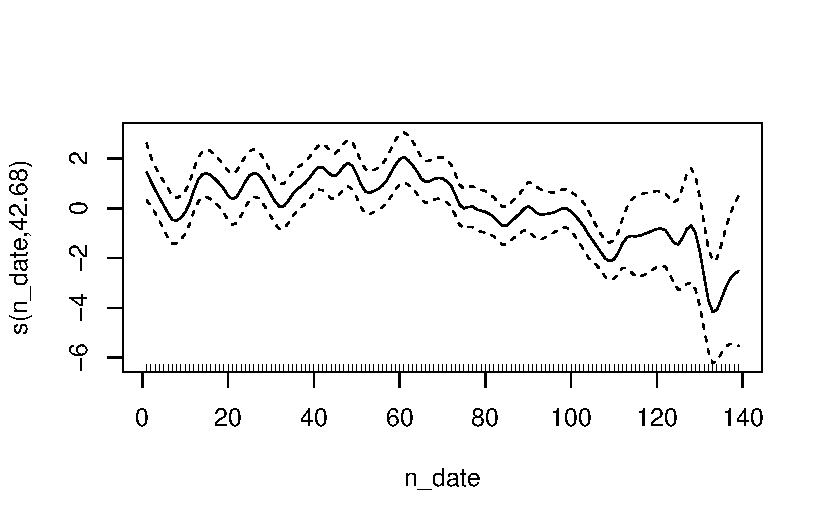
\includegraphics{dlm_gam_comparison_files/figure-pdf/unnamed-chunk-5-1.pdf}

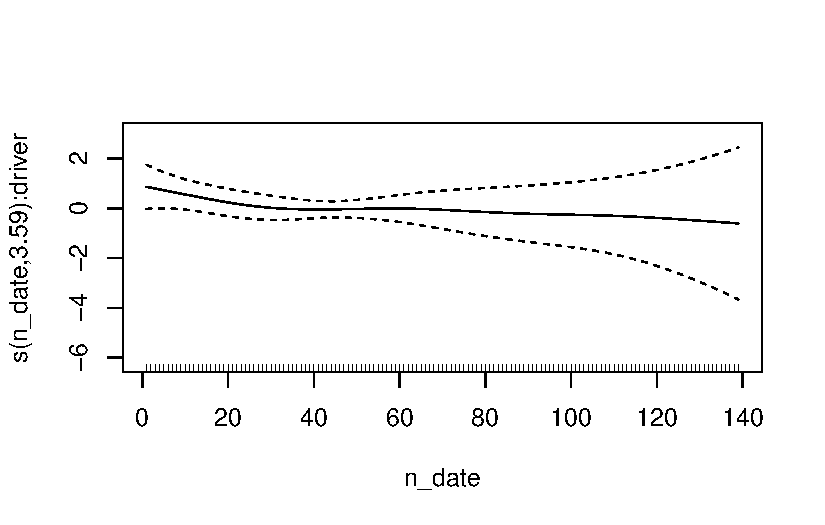
\includegraphics{dlm_gam_comparison_files/figure-pdf/unnamed-chunk-5-2.pdf}

\begin{Shaded}
\begin{Highlighting}[]
\NormalTok{plot\_2 }\OtherTok{\textless{}{-}} \FunctionTok{plot}\NormalTok{(gam\_lakewa\_2, }\AttributeTok{seWithMean =} \ConstantTok{TRUE}\NormalTok{, }\AttributeTok{n =} \FunctionTok{nrow}\NormalTok{(dat\_lakewa))}
\end{Highlighting}
\end{Shaded}

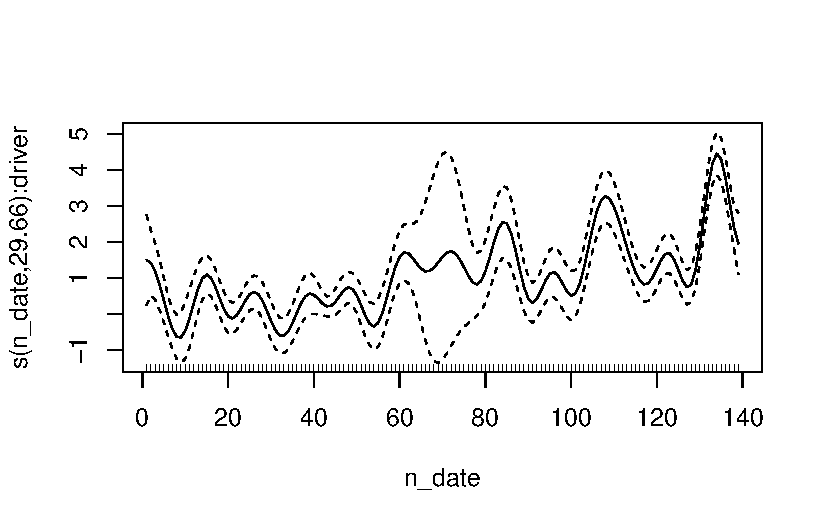
\includegraphics{dlm_gam_comparison_files/figure-pdf/unnamed-chunk-5-3.pdf}

\begin{Shaded}
\begin{Highlighting}[]
\NormalTok{plot\_3 }\OtherTok{\textless{}{-}} \FunctionTok{plot}\NormalTok{(gam\_aksalmon\_1, }\AttributeTok{seWithMean =} \ConstantTok{TRUE}\NormalTok{, }\AttributeTok{n =} \FunctionTok{nrow}\NormalTok{(dat\_aksalmon))}
\end{Highlighting}
\end{Shaded}

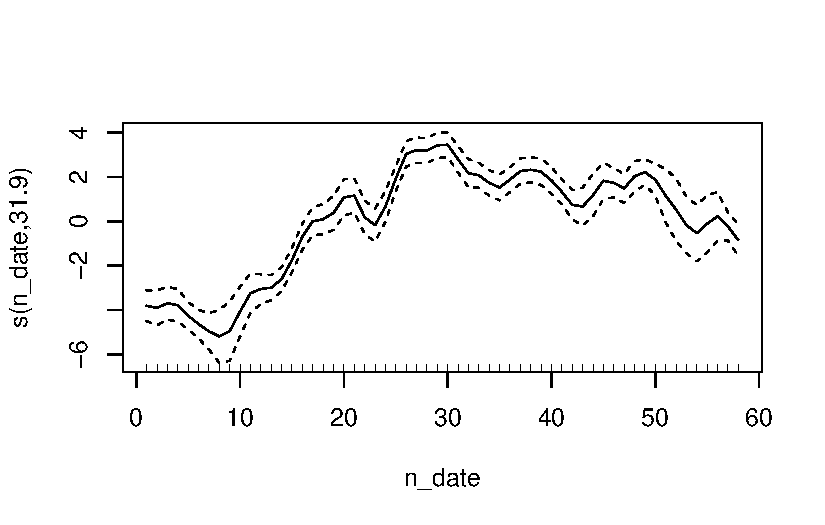
\includegraphics{dlm_gam_comparison_files/figure-pdf/unnamed-chunk-5-4.pdf}

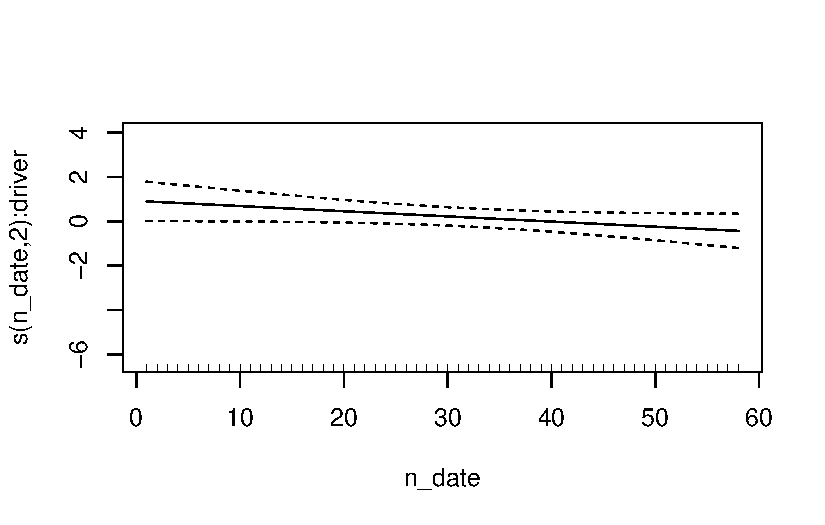
\includegraphics{dlm_gam_comparison_files/figure-pdf/unnamed-chunk-5-5.pdf}

\begin{Shaded}
\begin{Highlighting}[]
\NormalTok{plot\_4 }\OtherTok{\textless{}{-}} \FunctionTok{plot}\NormalTok{(gam\_aksalmon\_2, }\AttributeTok{seWithMean =} \ConstantTok{TRUE}\NormalTok{, }\AttributeTok{n =} \FunctionTok{nrow}\NormalTok{(dat\_aksalmon))}
\end{Highlighting}
\end{Shaded}

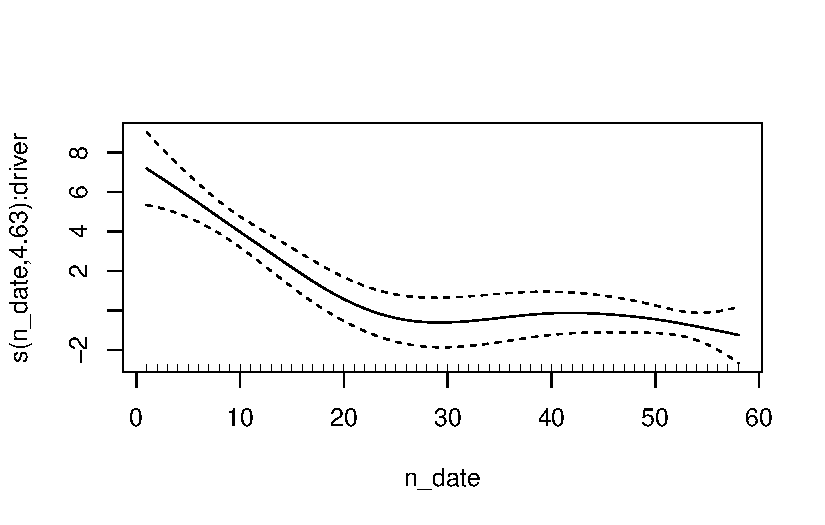
\includegraphics{dlm_gam_comparison_files/figure-pdf/unnamed-chunk-5-6.pdf}

\begin{Shaded}
\begin{Highlighting}[]
\NormalTok{dat\_aksalmon}\SpecialCharTok{$}\NormalTok{date }\OtherTok{\textless{}{-}} \FunctionTok{paste0}\NormalTok{(dat\_aksalmon}\SpecialCharTok{$}\NormalTok{date,}\StringTok{"{-}01{-}01"}\NormalTok{)}

\NormalTok{coef\_dlm\_lakeWA1 }\OtherTok{\textless{}{-}} \FunctionTok{data.frame}\NormalTok{(}\AttributeTok{date =}\NormalTok{ dat\_lakewa}\SpecialCharTok{$}\NormalTok{date, }
                        \AttributeTok{int\_est =}\NormalTok{ dlm\_lakewa\_1}\SpecialCharTok{$}\NormalTok{states[}\DecValTok{1}\NormalTok{,],}
                        \AttributeTok{int\_se =}\NormalTok{ dlm\_lakewa\_1}\SpecialCharTok{$}\NormalTok{states.se[}\DecValTok{1}\NormalTok{,],}
                        \AttributeTok{slope\_est =}\NormalTok{ dlm\_lakewa\_1}\SpecialCharTok{$}\NormalTok{states[}\DecValTok{2}\NormalTok{,],}
                        \AttributeTok{slope\_se =}\NormalTok{ dlm\_lakewa\_1}\SpecialCharTok{$}\NormalTok{states.se[}\DecValTok{2}\NormalTok{,],}
                        \AttributeTok{time\_varying =} \StringTok{"Intercept + slope"}\NormalTok{,}
                        \AttributeTok{dataset =} \StringTok{"Lake Washington : DLM"}\NormalTok{)}
\NormalTok{coef\_dlm\_lakeWA2 }\OtherTok{\textless{}{-}} \FunctionTok{data.frame}\NormalTok{(}\AttributeTok{date =}\NormalTok{ dat\_lakewa}\SpecialCharTok{$}\NormalTok{date, }
                        \AttributeTok{int\_est =} \ConstantTok{NA}\NormalTok{,}
                        \AttributeTok{int\_se =} \ConstantTok{NA}\NormalTok{,}
                        \AttributeTok{slope\_est =}\NormalTok{ dlm\_lakewa\_2}\SpecialCharTok{$}\NormalTok{states[}\DecValTok{2}\NormalTok{,],}
                        \AttributeTok{slope\_se =}\NormalTok{ dlm\_lakewa\_2}\SpecialCharTok{$}\NormalTok{states.se[}\DecValTok{2}\NormalTok{,],}
                        \AttributeTok{time\_varying =} \StringTok{"Slope"}\NormalTok{,}
                        \AttributeTok{dataset =} \StringTok{"Lake Washington : DLM"}\NormalTok{)}
\NormalTok{coef\_dlm\_AK1 }\OtherTok{\textless{}{-}} \FunctionTok{data.frame}\NormalTok{(}\AttributeTok{date =}\NormalTok{ dat\_aksalmon}\SpecialCharTok{$}\NormalTok{date,}
                        \AttributeTok{int\_est =}\NormalTok{ dlm\_aksalmon\_1}\SpecialCharTok{$}\NormalTok{states[}\DecValTok{1}\NormalTok{,],}
                        \AttributeTok{int\_se =}\NormalTok{ dlm\_aksalmon\_1}\SpecialCharTok{$}\NormalTok{states.se[}\DecValTok{1}\NormalTok{,],}
                        \AttributeTok{slope\_est =}\NormalTok{ dlm\_aksalmon\_1}\SpecialCharTok{$}\NormalTok{states[}\DecValTok{2}\NormalTok{,],}
                        \AttributeTok{slope\_se =}\NormalTok{ dlm\_aksalmon\_1}\SpecialCharTok{$}\NormalTok{states.se[}\DecValTok{2}\NormalTok{,],}
                        \AttributeTok{time\_varying =} \StringTok{"Intercept + slope"}\NormalTok{,}
                        \AttributeTok{dataset =} \StringTok{"Alaska salmon : DLM"}\NormalTok{)}
\NormalTok{coef\_dlm\_AK2 }\OtherTok{\textless{}{-}} \FunctionTok{data.frame}\NormalTok{(}\AttributeTok{date =}\NormalTok{ dat\_aksalmon}\SpecialCharTok{$}\NormalTok{date,}
                        \AttributeTok{int\_est =} \ConstantTok{NA}\NormalTok{,}
                        \AttributeTok{int\_se =} \ConstantTok{NA}\NormalTok{,}
                        \AttributeTok{slope\_est =}\NormalTok{ dlm\_aksalmon\_2}\SpecialCharTok{$}\NormalTok{states[}\DecValTok{2}\NormalTok{,],}
                        \AttributeTok{slope\_se =}\NormalTok{ dlm\_aksalmon\_2}\SpecialCharTok{$}\NormalTok{states.se[}\DecValTok{2}\NormalTok{,],}
                        \AttributeTok{time\_varying =} \StringTok{"Slope"}\NormalTok{,}
                        \AttributeTok{dataset =} \StringTok{"Alaska salmon : DLM"}\NormalTok{)}


\NormalTok{coef\_gam\_lakeWA1 }\OtherTok{\textless{}{-}} \FunctionTok{data.frame}\NormalTok{(}\AttributeTok{date =}\NormalTok{ dat\_lakewa}\SpecialCharTok{$}\NormalTok{date, }
                        \AttributeTok{int\_est =}\NormalTok{ plot\_1[[}\DecValTok{1}\NormalTok{]]}\SpecialCharTok{$}\NormalTok{fit,}
                        \AttributeTok{int\_se =}\NormalTok{ plot\_1[[}\DecValTok{1}\NormalTok{]]}\SpecialCharTok{$}\NormalTok{se,}
                        \AttributeTok{slope\_est =}\NormalTok{ plot\_1[[}\DecValTok{2}\NormalTok{]]}\SpecialCharTok{$}\NormalTok{fit,}
                        \AttributeTok{slope\_se =}\NormalTok{ plot\_1[[}\DecValTok{2}\NormalTok{]]}\SpecialCharTok{$}\NormalTok{se,}
                        \AttributeTok{time\_varying =} \StringTok{"Intercept + slope"}\NormalTok{,}
                        \AttributeTok{dataset =} \StringTok{"Lake Washington : GAM"}\NormalTok{)}
\NormalTok{coef\_gam\_lakeWA2 }\OtherTok{\textless{}{-}} \FunctionTok{data.frame}\NormalTok{(}\AttributeTok{date =}\NormalTok{ dat\_lakewa}\SpecialCharTok{$}\NormalTok{date, }
                        \AttributeTok{int\_est =} \ConstantTok{NA}\NormalTok{,}
                        \AttributeTok{int\_se =} \ConstantTok{NA}\NormalTok{,}
                        \AttributeTok{slope\_est =}\NormalTok{ plot\_2[[}\DecValTok{1}\NormalTok{]]}\SpecialCharTok{$}\NormalTok{fit,}
                        \AttributeTok{slope\_se =}\NormalTok{ plot\_2[[}\DecValTok{1}\NormalTok{]]}\SpecialCharTok{$}\NormalTok{se,}
                        \AttributeTok{time\_varying =} \StringTok{"Slope"}\NormalTok{,}
                        \AttributeTok{dataset =} \StringTok{"Lake Washington : GAM"}\NormalTok{)}
\NormalTok{coef\_gam\_AK1 }\OtherTok{\textless{}{-}} \FunctionTok{data.frame}\NormalTok{(}\AttributeTok{date =}\NormalTok{ dat\_aksalmon}\SpecialCharTok{$}\NormalTok{date,}
                        \AttributeTok{int\_est =}\NormalTok{ plot\_3[[}\DecValTok{1}\NormalTok{]]}\SpecialCharTok{$}\NormalTok{fit,}
                        \AttributeTok{int\_se =}\NormalTok{ plot\_3[[}\DecValTok{1}\NormalTok{]]}\SpecialCharTok{$}\NormalTok{fit,}
                        \AttributeTok{slope\_est =}\NormalTok{ plot\_3[[}\DecValTok{2}\NormalTok{]]}\SpecialCharTok{$}\NormalTok{fit,}
                        \AttributeTok{slope\_se =}\NormalTok{ plot\_3[[}\DecValTok{2}\NormalTok{]]}\SpecialCharTok{$}\NormalTok{fit,}
                        \AttributeTok{time\_varying =} \StringTok{"Intercept + slope"}\NormalTok{,}
                        \AttributeTok{dataset =} \StringTok{"Alaska salmon : GAM"}\NormalTok{)}
\NormalTok{coef\_gam\_AK2 }\OtherTok{\textless{}{-}} \FunctionTok{data.frame}\NormalTok{(}\AttributeTok{date =}\NormalTok{ dat\_aksalmon}\SpecialCharTok{$}\NormalTok{date,}
                        \AttributeTok{int\_est =} \ConstantTok{NA}\NormalTok{,}
                        \AttributeTok{int\_se =} \ConstantTok{NA}\NormalTok{,}
                        \AttributeTok{slope\_est =}\NormalTok{ plot\_4[[}\DecValTok{1}\NormalTok{]]}\SpecialCharTok{$}\NormalTok{fit,}
                        \AttributeTok{slope\_se =}\NormalTok{ plot\_4[[}\DecValTok{1}\NormalTok{]]}\SpecialCharTok{$}\NormalTok{se,}
                        \AttributeTok{time\_varying =} \StringTok{"Slope"}\NormalTok{,}
                        \AttributeTok{dataset =} \StringTok{"Alaska salmon : GAM"}\NormalTok{)}

\NormalTok{coefs }\OtherTok{\textless{}{-}} \FunctionTok{rbind}\NormalTok{(coef\_dlm\_lakeWA1, coef\_dlm\_lakeWA2, coef\_dlm\_AK1, coef\_dlm\_AK2,}
\NormalTok{               coef\_gam\_lakeWA1, coef\_gam\_lakeWA2, coef\_gam\_AK1, coef\_gam\_AK2)}

\FunctionTok{ggplot}\NormalTok{(coefs, }\FunctionTok{aes}\NormalTok{(date, slope\_est, }\AttributeTok{group =}\NormalTok{ time\_varying, }\AttributeTok{fill=}\NormalTok{time\_varying, }\AttributeTok{col=}\NormalTok{time\_varying)) }\SpecialCharTok{+} 
  \FunctionTok{geom\_ribbon}\NormalTok{(}\FunctionTok{aes}\NormalTok{(}\AttributeTok{ymin=}\NormalTok{slope\_est}\DecValTok{{-}2}\SpecialCharTok{*}\NormalTok{slope\_se, }\AttributeTok{ymax =}\NormalTok{ slope\_est}\SpecialCharTok{+}\DecValTok{2}\SpecialCharTok{*}\NormalTok{slope\_se), }\AttributeTok{alpha=}\FloatTok{0.3}\NormalTok{, }\AttributeTok{col =} \ConstantTok{NA}\NormalTok{) }\SpecialCharTok{+} 
  \FunctionTok{geom\_line}\NormalTok{(}\FunctionTok{aes}\NormalTok{(}\AttributeTok{lty=}\NormalTok{time\_varying)) }\SpecialCharTok{+} 
  \FunctionTok{ylab}\NormalTok{(}\StringTok{"Time{-}varying slope"}\NormalTok{) }\SpecialCharTok{+} 
  \FunctionTok{xlab}\NormalTok{(}\StringTok{""}\NormalTok{) }\SpecialCharTok{+} \FunctionTok{theme\_bw}\NormalTok{() }\SpecialCharTok{+} 
  \FunctionTok{facet\_wrap}\NormalTok{(}\SpecialCharTok{\textasciitilde{}}\NormalTok{ dataset, }\AttributeTok{scale=}\StringTok{"free"}\NormalTok{) }\SpecialCharTok{+} 
  \CommentTok{\#scale\_color\_viridis\_d(option="magma",begin=0.2, end=0.8, name = "Time{-}varying") + }
  \CommentTok{\#scale\_fill\_viridis\_d(option="magma",begin=0.2, end=0.8, name = "Time{-}varying") + }
  \FunctionTok{scale\_fill\_manual}\NormalTok{(}\AttributeTok{values=}\FunctionTok{c}\NormalTok{(col[}\DecValTok{4}\NormalTok{],col[}\DecValTok{5}\NormalTok{]))}\SpecialCharTok{+}
  \FunctionTok{scale\_colour\_manual}\NormalTok{(}\AttributeTok{values=}\FunctionTok{c}\NormalTok{(col[}\DecValTok{4}\NormalTok{],col[}\DecValTok{5}\NormalTok{]))}\SpecialCharTok{+}
  \FunctionTok{theme}\NormalTok{(}
    \AttributeTok{strip.background =} \FunctionTok{element\_rect}\NormalTok{(}\AttributeTok{fill =} \StringTok{"white"}\NormalTok{)}
\NormalTok{  )}
\end{Highlighting}
\end{Shaded}

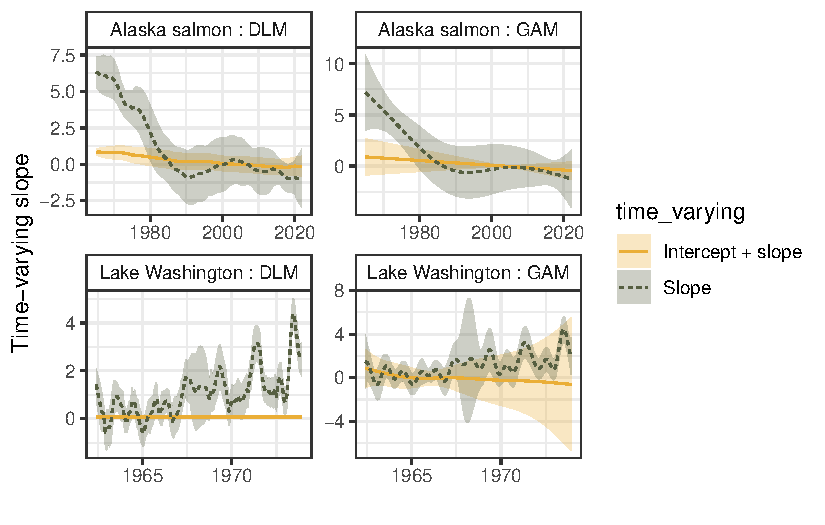
\includegraphics{dlm_gam_comparison_files/figure-pdf/unnamed-chunk-6-1.pdf}

\begin{Shaded}
\begin{Highlighting}[]
\FunctionTok{ggsave}\NormalTok{(}\StringTok{"Figure\_2\_dlmgam\_comparison.png"}\NormalTok{, }\AttributeTok{height =} \DecValTok{7}\NormalTok{, }\AttributeTok{width =} \DecValTok{7}\NormalTok{)}
\end{Highlighting}
\end{Shaded}




\end{document}
